\notechapter{N-20220405}{Fréchet Differentiability, Hessians, and Constrained Tests}

\section{Fréchet differentiability and complex differentiability}

Complex differentiability is much stronger than ordinary real differentiability.  In one real direction a limit may exist, whereas in the complex plane the difference quotient must have the same limit along every direction.

Consider
\[
  f(z)=\overline z,\qquad z=a+bi.
\]
The complex derivative would be
\[
  f'(z)=\lim_{h\to0}\frac{\overline{z+h}-\overline z}{h}=\lim_{h\to0}\frac{\overline h}{h}.
\]
Along the real direction \(h=c\to0\),
\[
  \frac{\overline h}{h}=\frac c c=1.
\]
Along the imaginary direction \(h=di\to0\),
\[
  \frac{\overline h}{h}=\frac{-di}{di}=-1.
\]
Along the diagonal direction \(h=c+ci\),
\[
  \frac{\overline h}{h}=\frac{c-ci}{c+ci}=-i.
\]
The directional limits disagree, so \(f(z)=\overline z\) is not complex differentiable.  This is the basic reason complex differentiability is rigid.

If \(f(z)=u(x,y)+iv(x,y)\), the Cauchy--Riemann equations are
\[
  u_x=v_y,\qquad u_y=-v_x.
\]
When these hold with suitable regularity, the complex derivative is
\[
  f'(z_0)=u_x(x_0,y_0)+iv_x(x_0,y_0).
\]

\section{Fréchet derivative}

Let \(V,W\) be normed vector spaces, and let \(U\subseteq V\) be open.  A function \(f:U\to W\) is Fréchet differentiable at \(x\in U\) if there exists a bounded linear operator \(A:V\to W\) such that
\[
  \lim_{\|h\|\to0}\frac{\|f(x+h)-f(x)-Ah\|_W}{\|h\|_V}=0.
\]
Equivalently,
\[
  f(x+h)=f(x)+Ah+o(\|h\|).
\]
The operator \(A\) is unique and is denoted
\[
  Df(x)=A.
\]

The note compares this with the Gâteaux differential.  If \(k=\varepsilon h\), then
\[
  f(x+\varepsilon h)=f(x)+\varepsilon(Df)h+h\,o(\varepsilon),
\]
and, in the limit, one gets a directional derivative.  But the Fréchet derivative is stronger: it requires one linear map to approximate the function uniformly in all directions.

\section{Visualizing complex maps}

The page shows conformal grid pictures: a rectangular grid is sent to curved orthogonal families under maps such as
\[
  f(z)=z^2,\qquad f(z)=\frac1z,\qquad f(z)=\sin z.
\]
The key geometric point is that holomorphic maps with nonzero derivative preserve angles locally.  They may bend the grid, but they preserve the orthogonality of the two coordinate families.

\begin{figure}[H]
\centering
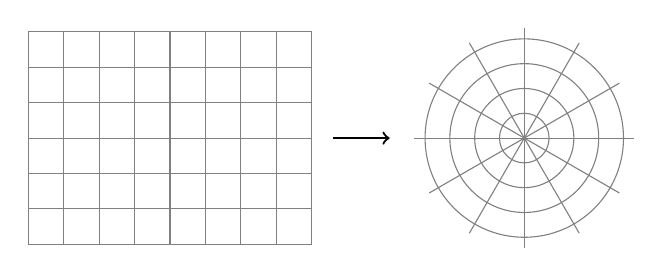
\begin{tikzpicture}[scale=0.9]
  \foreach \x in {-2,-1.5,...,2}{\draw[gray] (\x,-1.5)--(\x,1.5);}
  \foreach \y in {-1.5,-1,...,1.5}{\draw[gray] (-2,\y)--(2,\y);}
  \draw[->,thick] (2.3,0)--(3.1,0);
  \begin{scope}[xshift=5cm]
    \foreach \r in {0.35,0.7,1.05,1.4}{\draw[gray] (0,0) circle (\r);}
    \foreach \a in {0,30,...,330}{\draw[gray] (0,0)--(\a:1.55);}
  \end{scope}
\end{tikzpicture}
\caption{Schematic reconstruction: a rectangular grid is deformed into orthogonal curve families by a holomorphic map.}
\end{figure}

\section{Hessian matrices and Taylor expansion}

The second main topic is the relationship between Hessians, Taylor expansion, and extrema.  For a smooth function \(f:\mathbb R^n\to\mathbb R\), Taylor expansion at a critical point \(p\) gives
\[
  f(p+h)=f(p)+\frac12 h^T H_f(p)h+O(\|h\|^3).
\]
Thus the quadratic form associated to the Hessian controls the local behavior.

For unconstrained extrema, positive definiteness of \(H_f(p)\) gives a local minimum, negative definiteness gives a local maximum, and indefiniteness gives a saddle.  For constrained extrema the situation is subtler, because one must restrict the second variation to the tangent space of the constraint.

\section{Bordered Hessian}

For a constrained problem
\[
  \text{extremize }f(x)\quad\text{subject to }g_1(x)=\cdots=g_m(x)=0,
\]
one introduces the Lagrangian
\[
  \mathcal L(x,\lambda)=f(x)-\sum_{i=1}^m\lambda_i g_i(x).
\]
The bordered Hessian packages the second derivatives of \(\mathcal L\) together with the first derivatives of the constraints:
\[
  H_B=
  \begin{pmatrix}
  0 & Dg\\
  Dg^T & D_x^2\mathcal L
  \end{pmatrix}.
\]
The sign pattern of certain principal minors then diagnoses constrained maxima and minima.

\section{Example}

The note considers the inequality problem
\[
  a,b,c>0,\qquad ab+bc+ca=a+b+c,
\]
and asks to prove
\[
  \sqrt{ab}+\sqrt{bc}+\sqrt{ca}-\sqrt{abc}\ge2.
\]
Let
\[
  f(a,b,c)=\sqrt{ab}+\sqrt{bc}+\sqrt{ca}-\sqrt{abc},
\]
and
\[
  g(a,b,c)=a+b+c-ab-bc-ca.
\]
The Lagrangian is
\[
  F(a,b,c,\lambda)=f(a,b,c)+\lambda g(a,b,c).
\]
The first-order equations are
\[
\begin{cases}
\displaystyle \frac{\sqrt{abc}-\sqrt{ab}+\sqrt{ac}}{2a}+\lambda(1-b-c)=0,\\
\displaystyle \frac{\sqrt{abc}+\sqrt{ab}+\sqrt{bc}}{2b}+\lambda(1-a-c)=0,\\
\displaystyle \frac{\sqrt{abc}+\sqrt{ac}+\sqrt{bc}}{2c}+\lambda(1-a-b)=0,\\
a+b+c-ab-bc-ca=0.
\end{cases}
\]
The symmetric point
\[
  a=b=c=1
\]
is a critical point.  At that point the bordered Hessian has the schematic form
\[
  H_B=
  \begin{pmatrix}
  0&-1&-1&-1\\
  -1&-\frac14&0&0\\
  -1&0&-\frac14&0\\
  -1&0&0&-\frac14
  \end{pmatrix}.
\]
The relevant minors have the required sign pattern, so the symmetric point gives the constrained extremum.  Since
\[
  f(1,1,1)=2,
\]
we obtain the desired inequality.

\section{Finite fields and Galois theory}

A final aside in the note jumps to finite fields and Galois theory.  The basic facts listed are:
\begin{enumerate}[(i)]
  \item the finite field \(\mathbb F_p\) has arithmetic modulo \(p\);
  \item polynomial factorization over \(\mathbb F_p\) can differ dramatically from factorization over \(\mathbb Q\);
  \item adjoining roots creates finite extensions such as \(\mathbb F_{p^n}\);
  \item quotient rings \(\mathbb F_p[x]/(q(x))\) construct finite fields when \(q\) is irreducible.

\end{enumerate}
Thus the same algebraic idea reappears: to solve an equation, enlarge the field, then study the symmetries of the roots.

\section{Why complex analysis meets Hessians}

Complex differentiability and Hessian tests share a common theme: first-order information determines the allowed linear approximation, while second-order information controls what happens after the first-order obstruction vanishes.

For \(f(z)=\overline z\), the real derivative exists as a real-linear map, but complex differentiability asks for multiplication by one complex number.  The failure is exactly the failure of a real-linear map to commute with multiplication by \(i\).  In modern language, complex differentiability means the derivative is \(\mathbb C\)-linear, not merely \(\mathbb R\)-linear.

For constrained extrema, the first-order condition removes the tangent freedom, so the Hessian test must be performed only on tangent directions to the constraint.  This is why the bordered Hessian appears: it is not a mysterious determinant recipe, but a bookkeeping device for second variation under first-order constraints.


\section{Frechet derivative as linear approximation}

For a map \(F:V\to W\) between normed spaces, differentiability at \(a\) means there is a bounded linear map \(L\) such that
\[
  F(a+h)=F(a)+Lh+o(\|h\|).
\]
This \(L\) is the Frechet derivative.  It is stronger and cleaner than checking directional derivatives separately, because it requires one linear map to approximate the function uniformly in all directions.

\section{Hessian as second derivative}

For scalar-valued functions, the Hessian is the derivative of the gradient.  It records the quadratic part of the Taylor expansion:
\[
  f(a+h)=f(a)+Df(a)h+\frac12 h^T H_f(a)h+o(\|h\|^2).
\]
At a critical point, the linear term vanishes, so the Hessian controls the first visible local shape.
